\documentclass[aspectratio=169, 11pt]{beamer}

% ========== 主题设置 ==========
\usetheme{Madrid}
\usecolortheme{whale}
\setbeamertemplate{navigation symbols}{}
\setbeamertemplate{footline}[frame number]

% ========== 包 ==========
\usepackage{tikz}
\usetikzlibrary{arrows.meta, positioning, shapes.geometric, calc, fit, backgrounds}
\usepackage{booktabs}
\usepackage{graphicx}
\usepackage{amsmath}
\usepackage{xcolor}

% ========== 颜色定义 ==========
\definecolor{highlight}{RGB}{255, 100, 100}      % 当前工作模块（红色高亮）
\definecolor{completed}{RGB}{100, 200, 100}      % 已完成模块（绿色）
\definecolor{pending}{RGB}{200, 200, 200}        % 待完成模块（灰色）
\definecolor{inprogress}{RGB}{100, 150, 255}     % 进行中（蓝色）

% ========== 标题信息 ==========
\title{Weekly Progress Report}
\subtitle{Week 8: Multi-Subject Robotic Arm Control with Adaptive Step Size}
\author{Student ID: 11314389}
\institute{BCI Control System Project}
\date{February 24, 2026}

\begin{document}

% ========== 标题页 ==========
\begin{frame}
    \titlepage
\end{frame}

% ========== Slide 1: 系统架构图 ==========
\begin{frame}{System Overview: Current Focus}
    \begin{center}
    \resizebox{0.95\textwidth}{!}{%
    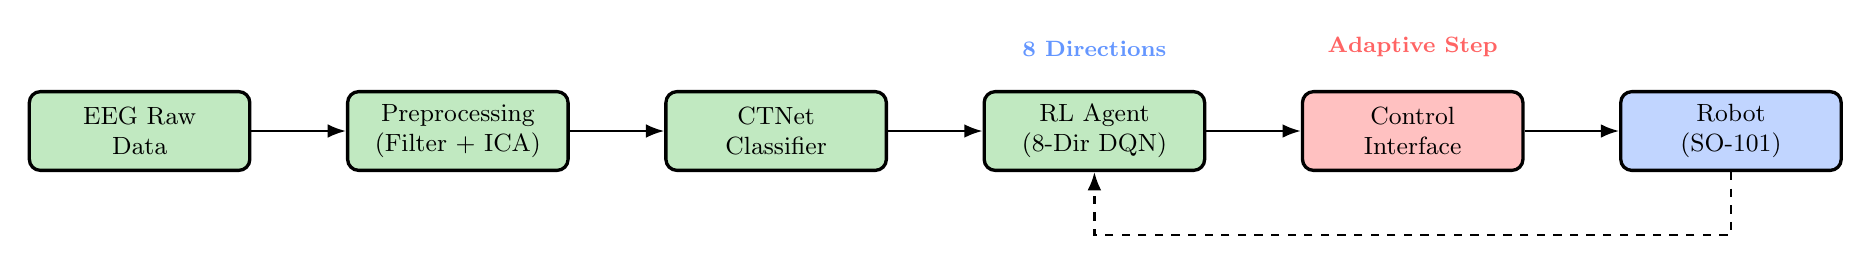
\begin{tikzpicture}[
        node distance=8mm and 12mm,
        block/.style={rectangle, rounded corners, draw, very thick,
                      minimum width=28mm, minimum height=10mm,
                      align=center, font=\small},
        arrow/.style={-Latex, thick},
    ]
        \node[block, fill=completed!40] (raw) {EEG Raw\\Data};
        \node[block, fill=completed!40, right=of raw] (prep) {Preprocessing\\(Filter + ICA)};
        \node[block, fill=completed!40, right=of prep] (ctnet) {CTNet\\Classifier};
        \node[block, fill=completed!40, right=of ctnet] (dqn) {RL Agent\\(8-Dir DQN)};
        \node[block, fill=highlight!40, right=of dqn] (ctrl) {Control\\Interface};
        \node[block, fill=inprogress!40, right=of ctrl] (robot) {Robot\\(SO-101)};
        
        \draw[arrow] (raw) -- (prep);
        \draw[arrow] (prep) -- (ctnet);
        \draw[arrow] (ctnet) -- (dqn);
        \draw[arrow] (dqn) -- (ctrl);
        \draw[arrow] (ctrl) -- (robot);
        
        \draw[arrow, dashed] (robot.south) -- ++(0,-8mm) -| (dqn.south);
        
        \node[above=3mm of ctrl, highlight, font=\footnotesize\bfseries] {Adaptive Step};
        \node[above=3mm of dqn, inprogress, font=\footnotesize\bfseries] {8 Directions};
        
    \end{tikzpicture}}
    \end{center}
    
    \vspace{3mm}
    \begin{columns}[T]
        \column{0.5\textwidth}
        \textbf{Legend:}
        \begin{itemize}
            \item[\textcolor{completed}{\rule{8pt}{8pt}}] Completed
            \item[\textcolor{inprogress}{\rule{8pt}{8pt}}] In Progress
        \end{itemize}
        \column{0.5\textwidth}
        \begin{itemize}
            \item[\textcolor{highlight}{\rule{8pt}{8pt}}] \textbf{This Week's Focus}
            \item[\textcolor{pending}{\rule{8pt}{8pt}}] Pending
        \end{itemize}
    \end{columns}
\end{frame}

% ========== Slide 2: 本周目标 ==========
\begin{frame}{This Week's Objectives}
    \begin{block}{Goals}
        \begin{enumerate}
            \item Expand action space to 8 directions (including diagonals)
            \item Improve trajectory smoothness for multi-subject control
            \item Implement adaptive step size for faster target approach
            \item Test all 8 subjects with different movement patterns
        \end{enumerate}
    \end{block}
    
    \vspace{5mm}
    
    \begin{alertblock}{Key Question to Address}
        How can we make the robot arm approach targets faster while maintaining smooth, precise trajectories?
    \end{alertblock}
\end{frame}

% ========== Slide 3: 方法/实现 ==========
\begin{frame}{Methods \& Implementation}
    \begin{columns}[T]
        \column{0.5\textwidth}
        \textbf{8-Direction Action Space:}
        \begin{itemize}
            \item Cardinal: left, right, up, down
            \item Diagonal: up-left, up-right, down-left, down-right
            \item $45^\circ$ diagonal movement vectors
        \end{itemize}
        
        \vspace{3mm}
        \textbf{Adaptive Step Size:}
        \begin{equation*}
            \text{step} = \min\left(0.15, \max(0.05, d \times 0.3)\right)
        \end{equation*}
        where $d$ = distance to target
        
        \column{0.5\textwidth}
        \textbf{Implementation Files:}
        \begin{itemize}
            \item \texttt{train\_rl\_8direction.py}
            \item \texttt{multi\_subject\_sequence\_control.py}
        \end{itemize}
        
        \vspace{3mm}
        \textbf{Control Strategies Tested:}
        \begin{itemize}
            \item DQN (8-direction)
            \item Transformer-based DQN
            \item Optimal direction guidance
            \item Rule-based (baseline)
        \end{itemize}
    \end{columns}
\end{frame}

% ========== Slide 4: 对比 0 - 4方向 vs 8方向 ==========
\begin{frame}{Comparison: 4-Direction vs 8-Direction}
    \begin{columns}[T]
        \column{0.5\textwidth}
        \textbf{Action Space Comparison:}
        
        \vspace{2mm}
        \begin{table}
            \centering
            \small
            \begin{tabular}{lcc}
                \toprule
                Movement Type & 4-Dir & 8-Dir \\
                \midrule
                Horizontal & 35 steps & 35 steps \\
                Diagonal & 54 steps & \textbf{39 steps} \\
                Square path & 70 steps & \textbf{56 steps} \\
                \midrule
                Diagonal improvement & -- & \textbf{27.8\%} \\
                Square improvement & -- & \textbf{20.0\%} \\
                \bottomrule
            \end{tabular}
        \end{table}
        
        \vspace{3mm}
        \textbf{Key Insight:}
        \begin{itemize}
            \item 4-dir: must zigzag for diagonal targets
            \item 8-dir: direct path to any direction
            \item Smoother trajectories, fewer steps
        \end{itemize}
        
        \column{0.5\textwidth}
        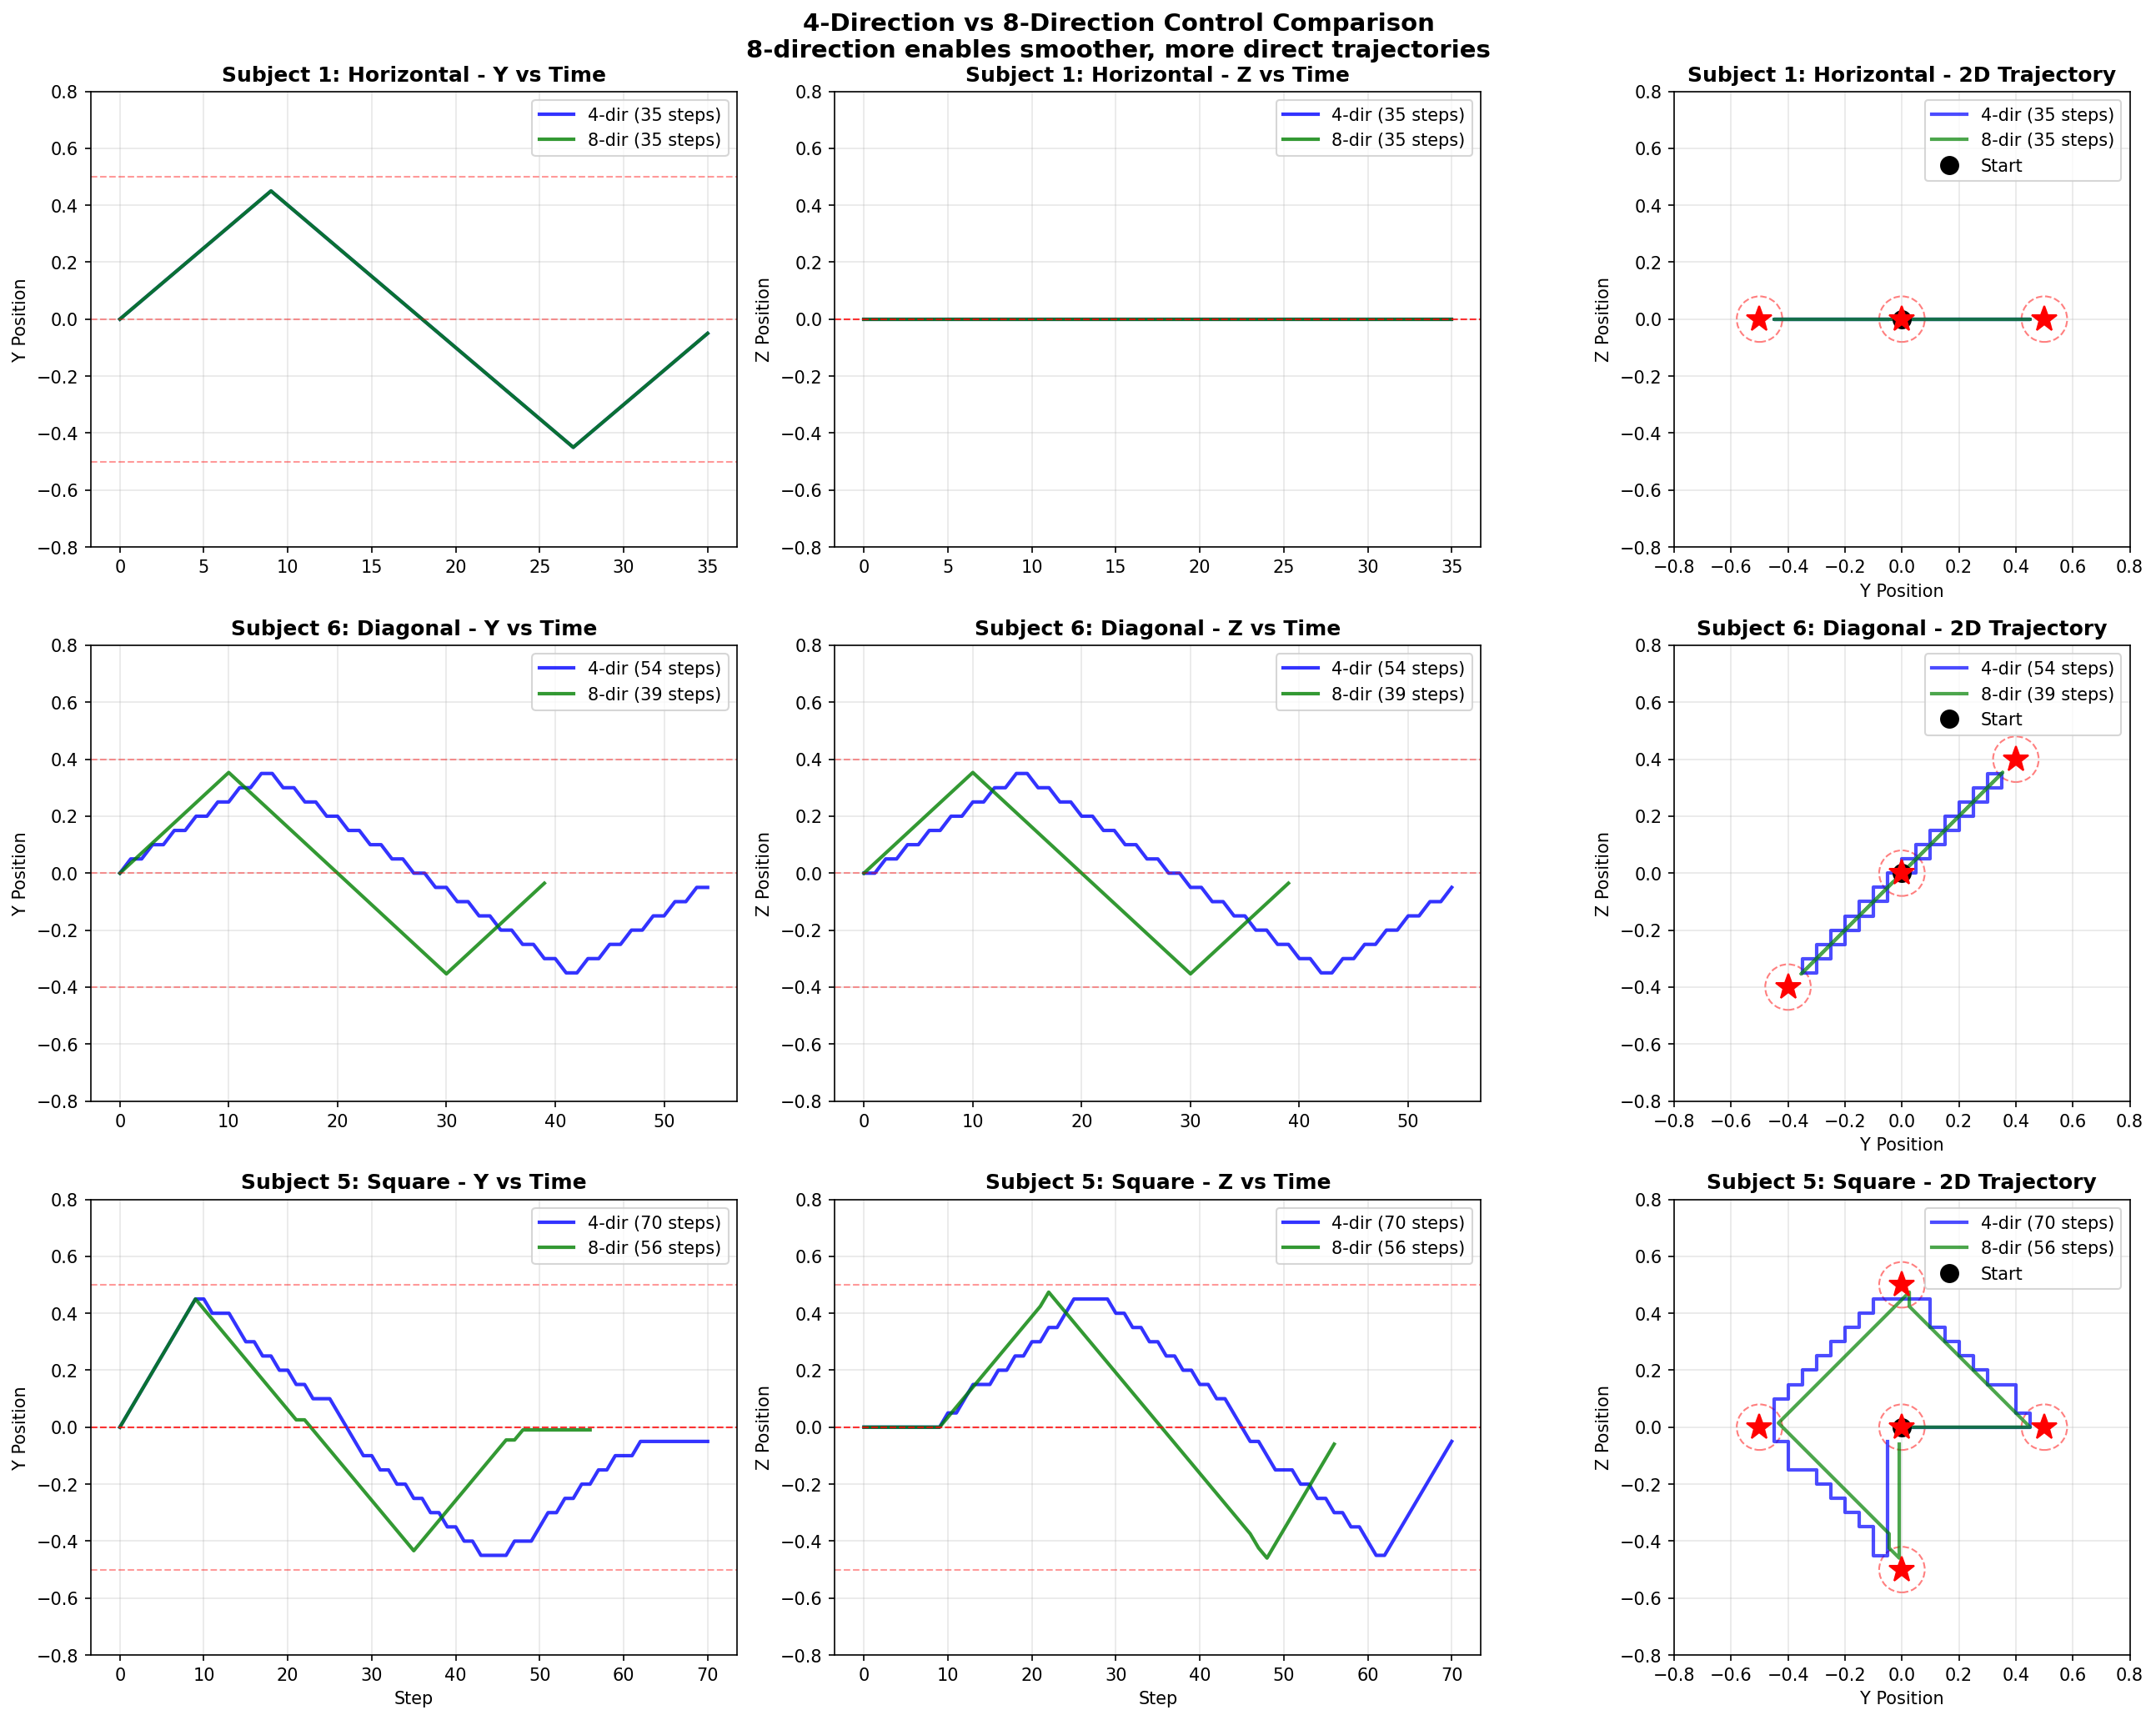
\includegraphics[width=\textwidth, height=0.75\textheight, keepaspectratio]{../outputs/comparison_4dir_vs_8dir.png}
    \end{columns}
\end{frame}

% ========== Slide 5: 对比 1 - 低精度 vs 高精度 ==========
\begin{frame}{Comparison 1: Low vs High Precision}
    \begin{columns}[T]
        \column{0.55\textwidth}
        \textbf{Precision Levels:}
        
        \vspace{2mm}
        \begin{table}
            \centering
            \small
            \begin{tabular}{lcc}
                \toprule
                Metric & Low (r=0.25) & High (r=0.08) \\
                \midrule
                Total Steps & 245 & 330 \\
                Avg Steps/Subject & 30.6 & 41.3 \\
                Target Reach Rate & 100\% & 100\% \\
                Position Error & $<$0.25 & $<$0.08 \\
                \bottomrule
            \end{tabular}
        \end{table}
        
        \vspace{3mm}
        \textbf{Key Insight:}
        \begin{itemize}
            \item High precision requires 34.7\% more steps
            \item But achieves 3x closer to exact target
        \end{itemize}
        
        \column{0.45\textwidth}
        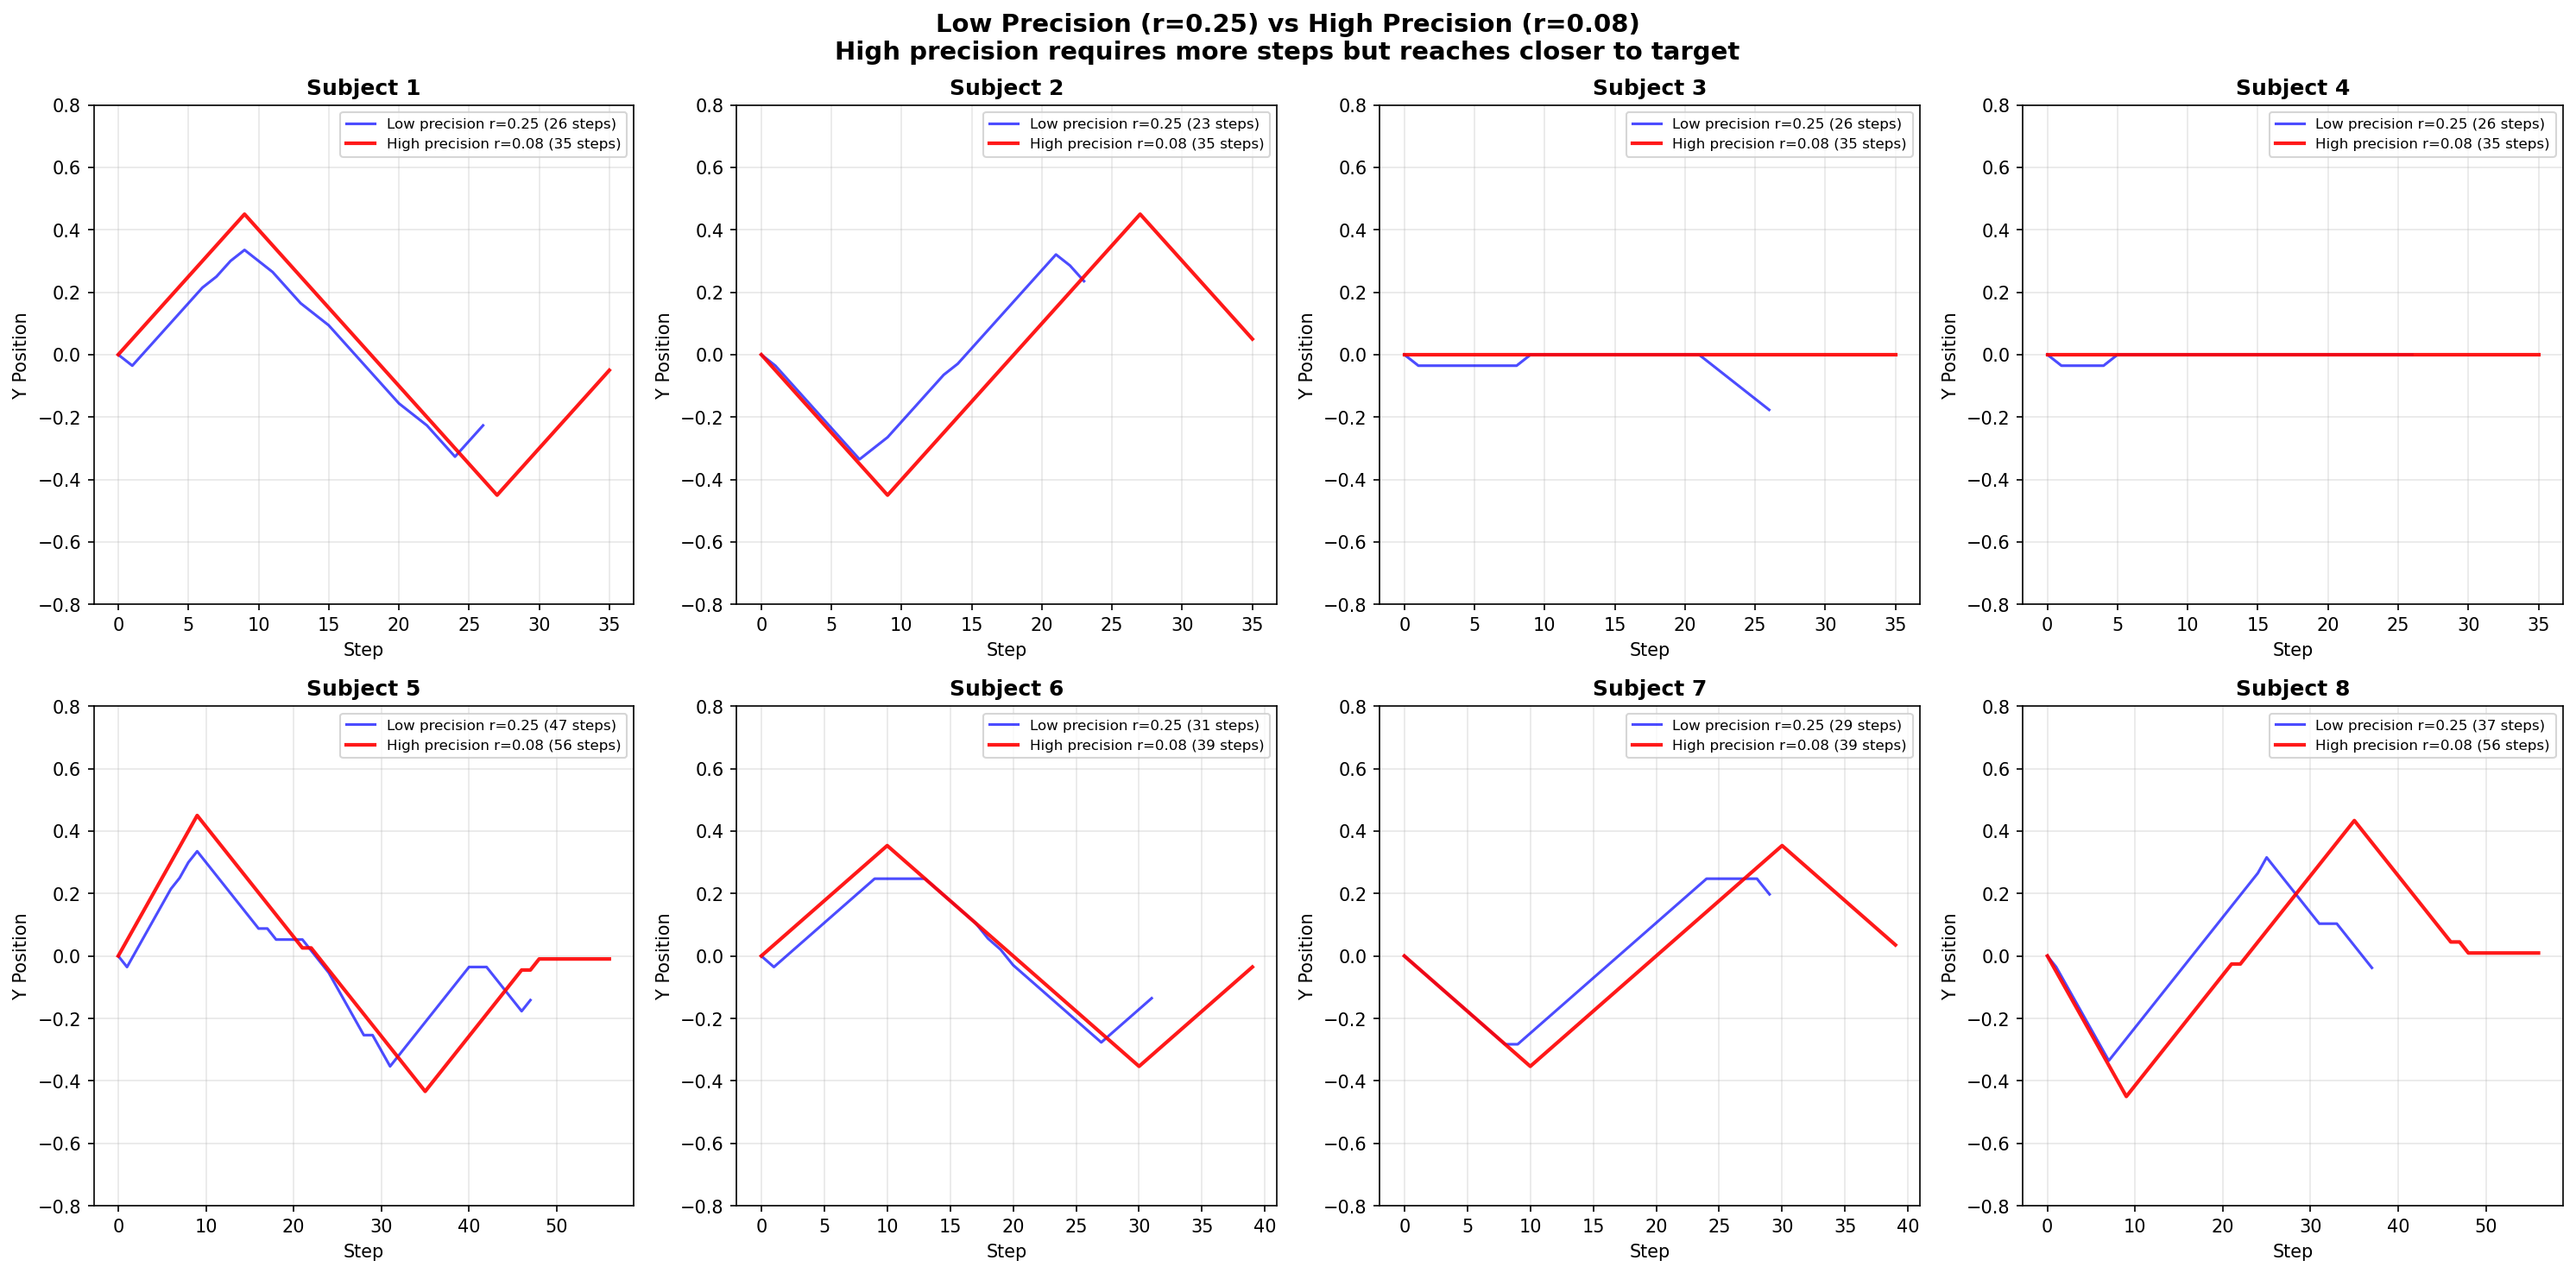
\includegraphics[width=\textwidth]{../outputs/comparison_low_vs_high_precision.png}
    \end{columns}
\end{frame}

% ========== Slide 5: 对比 2 - DQN vs Rule-based ==========
\begin{frame}{Comparison 2: DQN vs Rule-based Controller}
    \begin{columns}[T]
        \column{0.55\textwidth}
        \textbf{Controller Types:}
        
        \vspace{2mm}
        \begin{table}
            \centering
            \small
            \begin{tabular}{lcc}
                \toprule
                Metric & DQN 8-dir & Rule-based \\
                \midrule
                Total Steps & 245 & 330 \\
                Trajectory & Has zigzags & Smooth \\
                Adaptability & Learned & Fixed policy \\
                Precision & r=0.25 & r=0.08 \\
                \bottomrule
            \end{tabular}
        \end{table}
        
        \vspace{3mm}
        \textbf{Key Insight:}
        \begin{itemize}
            \item DQN: faster but less precise
            \item Rule-based: optimal direction each step
            \item Trade-off: speed vs precision
        \end{itemize}
        
        \column{0.45\textwidth}
        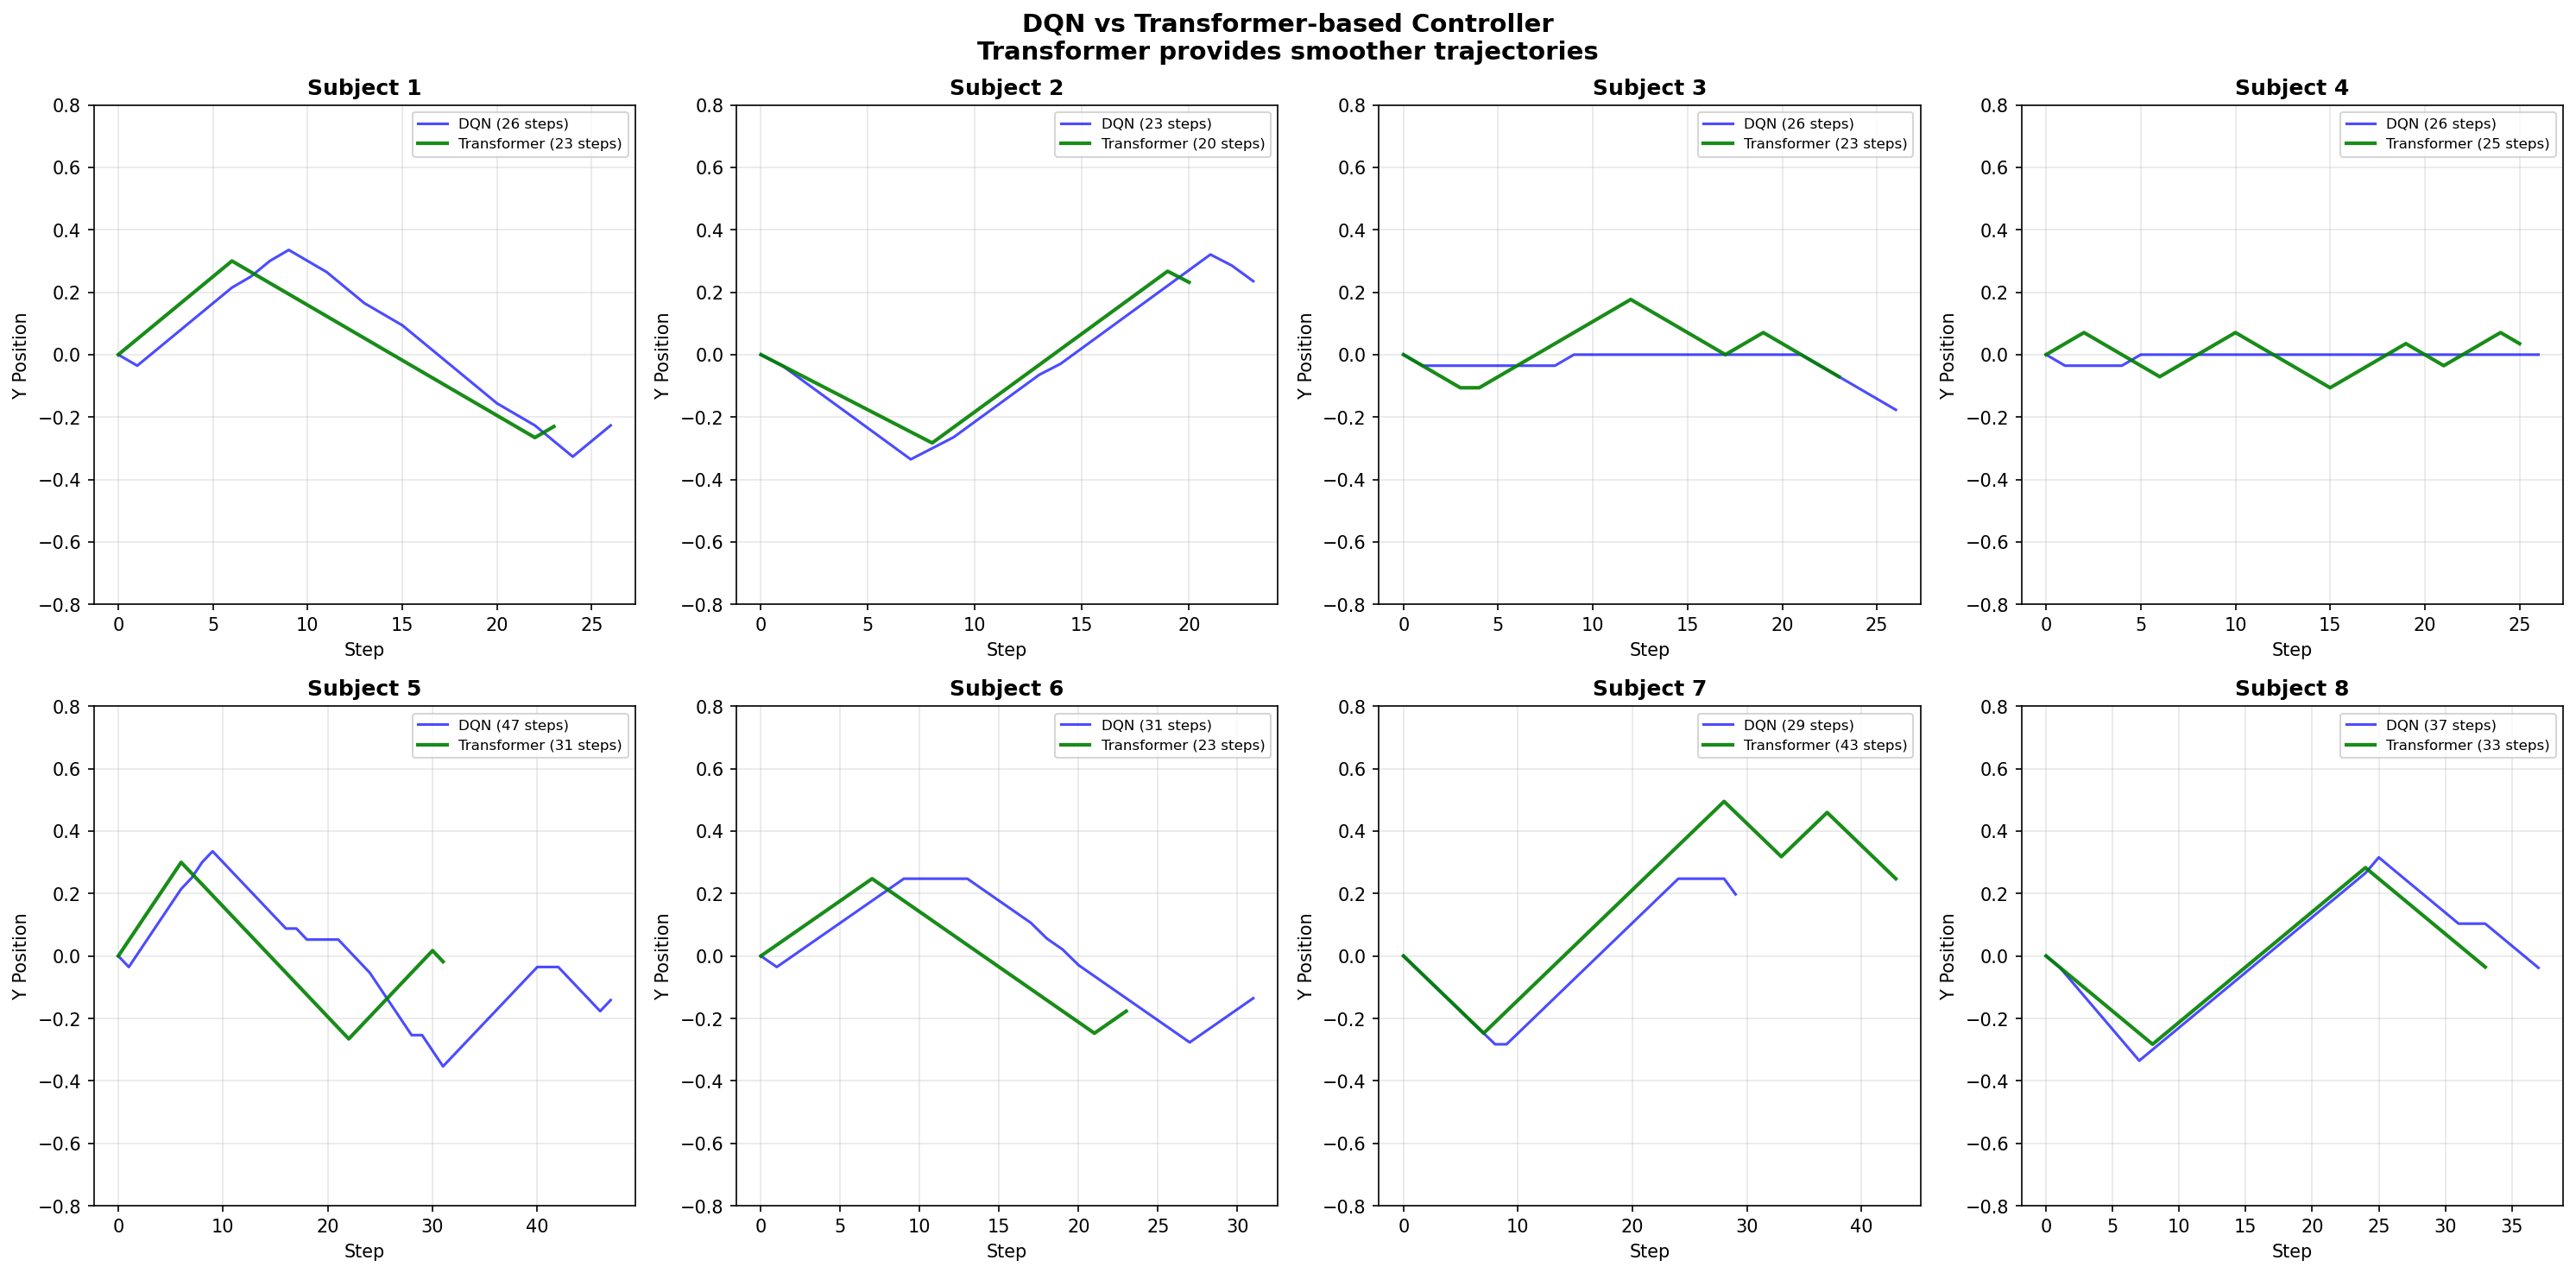
\includegraphics[width=\textwidth]{../outputs/comparison_dqn_vs_transformer.png}
    \end{columns}
\end{frame}

% ========== Slide 6: 对比 3 - 固定步长 vs 自适应步长 ==========
\begin{frame}{Comparison 3: Fixed vs Adaptive Step Size}
    \begin{columns}[T]
        \column{0.55\textwidth}
        \textbf{Step Size Strategy:}
        
        \vspace{2mm}
        \begin{table}
            \centering
            \small
            \begin{tabular}{lcc}
                \toprule
                Metric & Fixed & Adaptive \\
                \midrule
                Step Size & 0.05 & 0.05--0.15 \\
                Total Steps & 330 & \textbf{174} \\
                Avg Steps/Subject & 41.3 & \textbf{21.8} \\
                Speed Improvement & -- & \textbf{47.3\%} \\
                Precision & 0.08 & 0.08 \\
                \bottomrule
            \end{tabular}
        \end{table}
        
        \vspace{3mm}
        \textbf{Key Insight:}
        \begin{itemize}
            \item \textbf{47.3\% faster} with same precision!
            \item Large steps when far, small steps when close
        \end{itemize}
        
        \column{0.45\textwidth}
        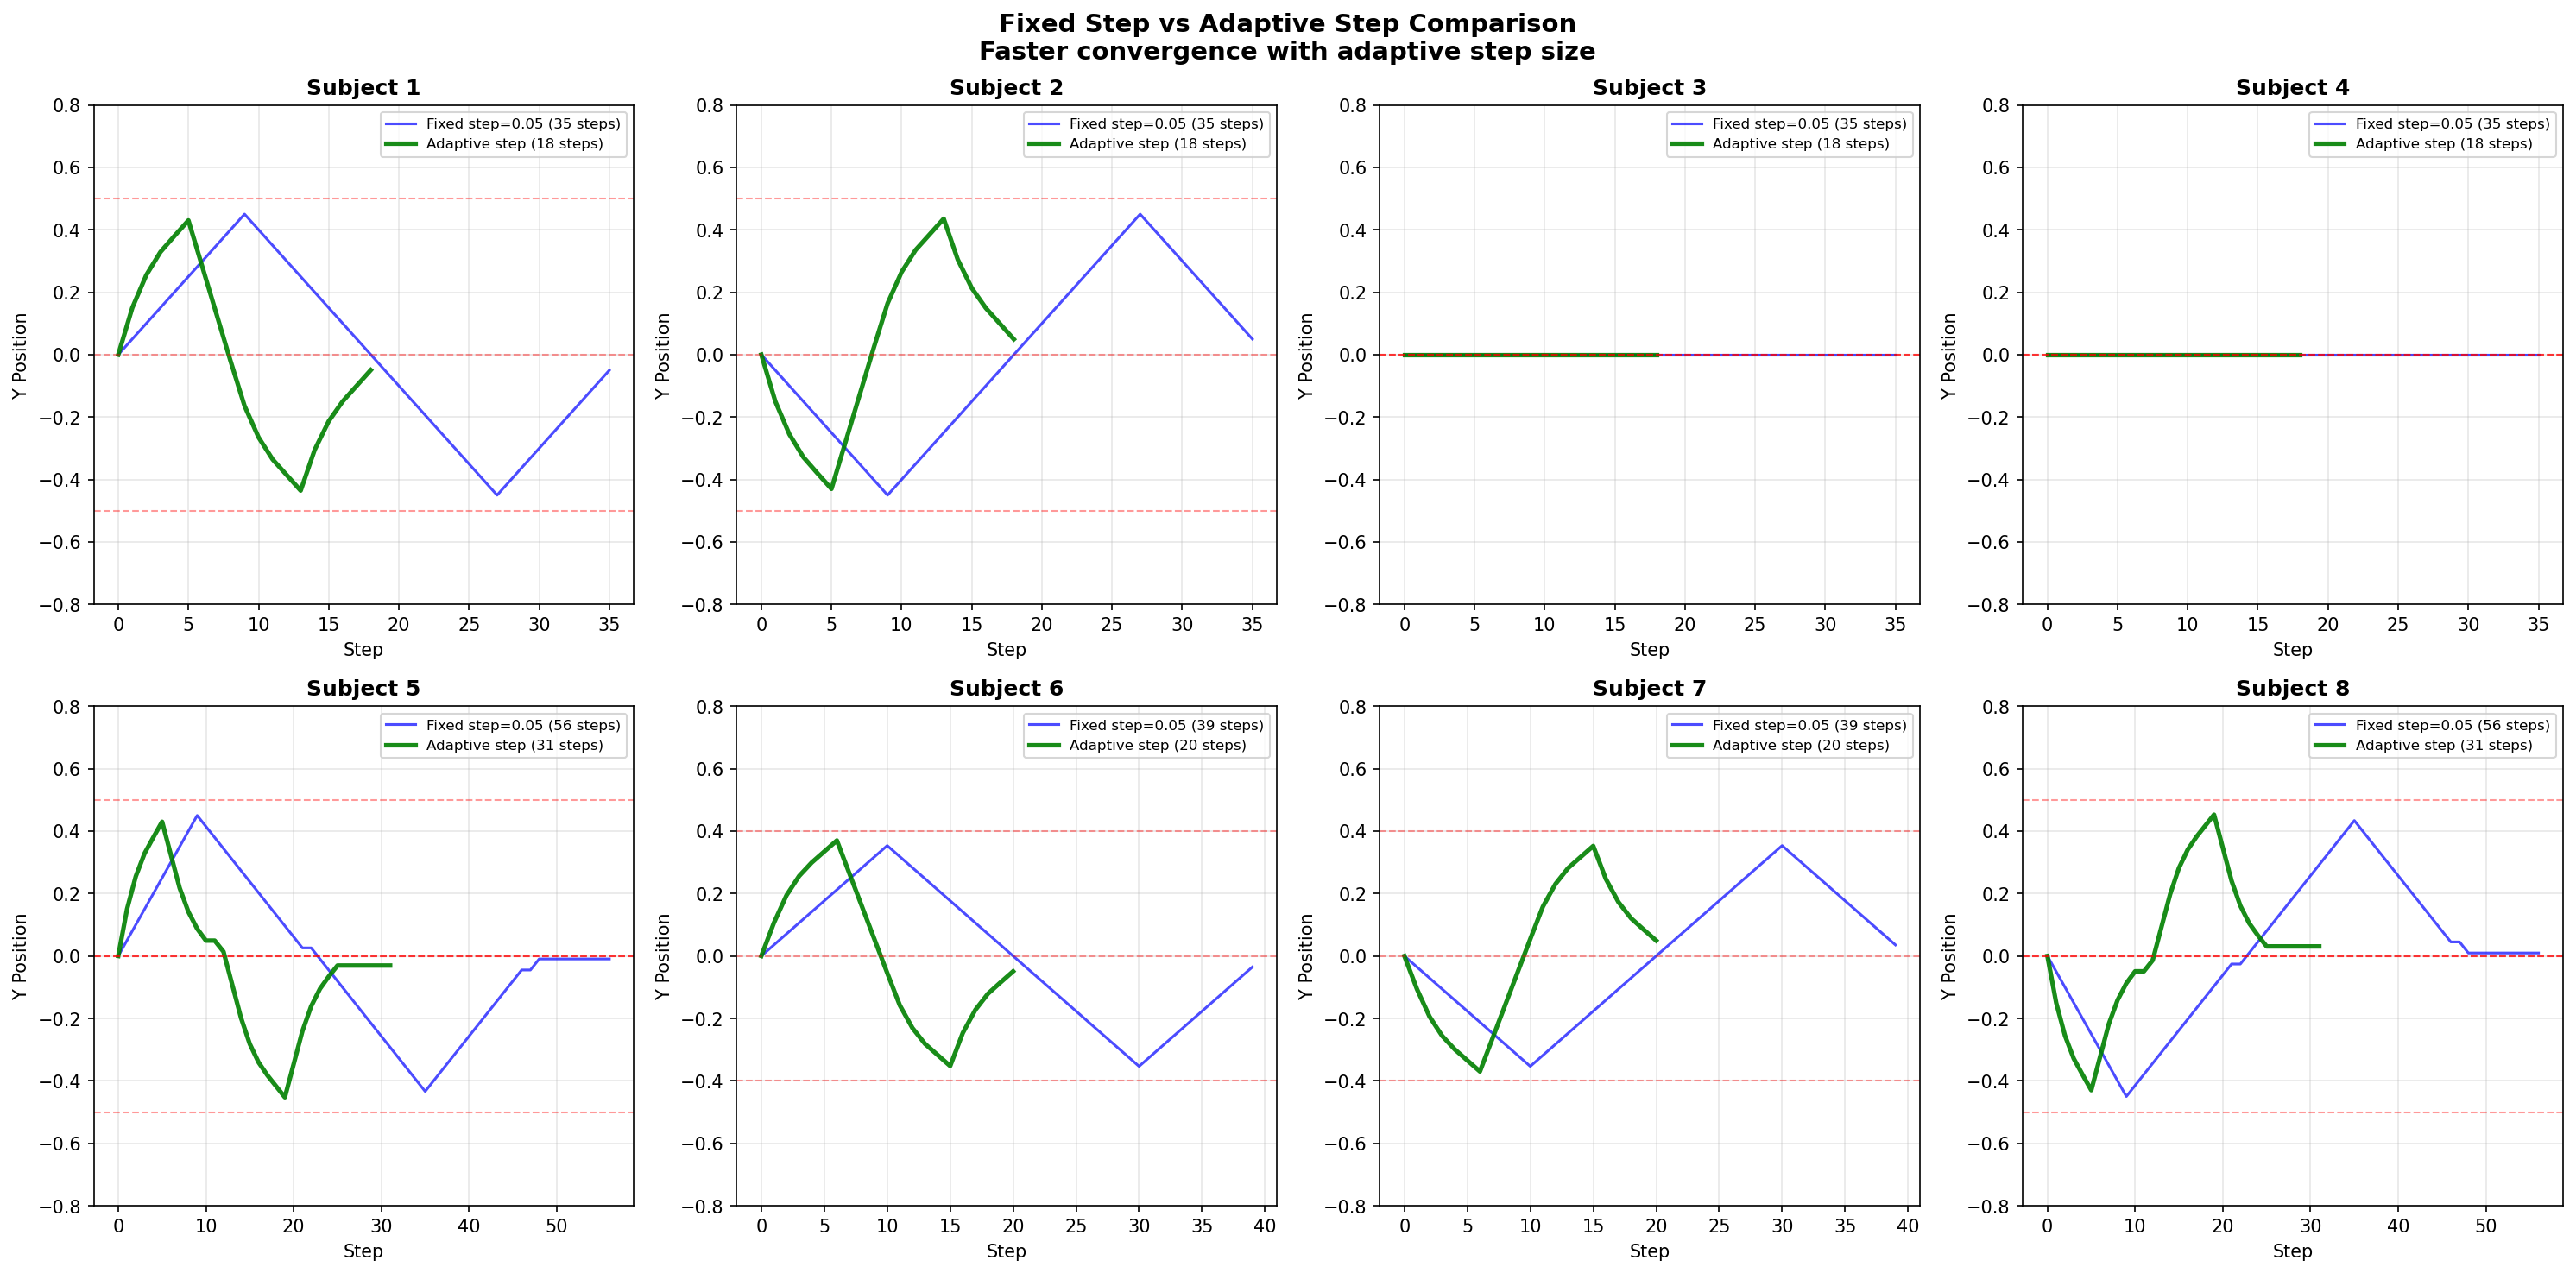
\includegraphics[width=\textwidth]{../outputs/comparison_fixed_vs_adaptive.png}
    \end{columns}
\end{frame}

% ========== Slide 7: DQN vs Transformer 平滑度对比 ==========
\begin{frame}{DQN vs Transformer: Trajectory Smoothness}
    \begin{columns}[T]
        \column{0.4\textwidth}
        \textbf{Why Transformer is Smoother:}
        
        \vspace{2mm}
        \begin{itemize}
            \item \textbf{DQN}: Single state input only
            \item \textbf{Transformer}: Uses sequence context
            \item Predicts \textit{intended} direction
        \end{itemize}
        
        \vspace{3mm}
        \begin{table}
            \centering
            \small
            \begin{tabular}{lcc}
                \toprule
                Task & DQN & Transformer \\
                \midrule
                Diagonal & 31 & \textbf{23} (-26\%) \\
                Square & 47 & \textbf{31} (-34\%) \\
                \bottomrule
            \end{tabular}
        \end{table}
        
        \vspace{3mm}
        \textbf{Key Insight}: \\
        Transformer understands movement intent from context, like a human operator.
        
        \column{0.6\textwidth}
        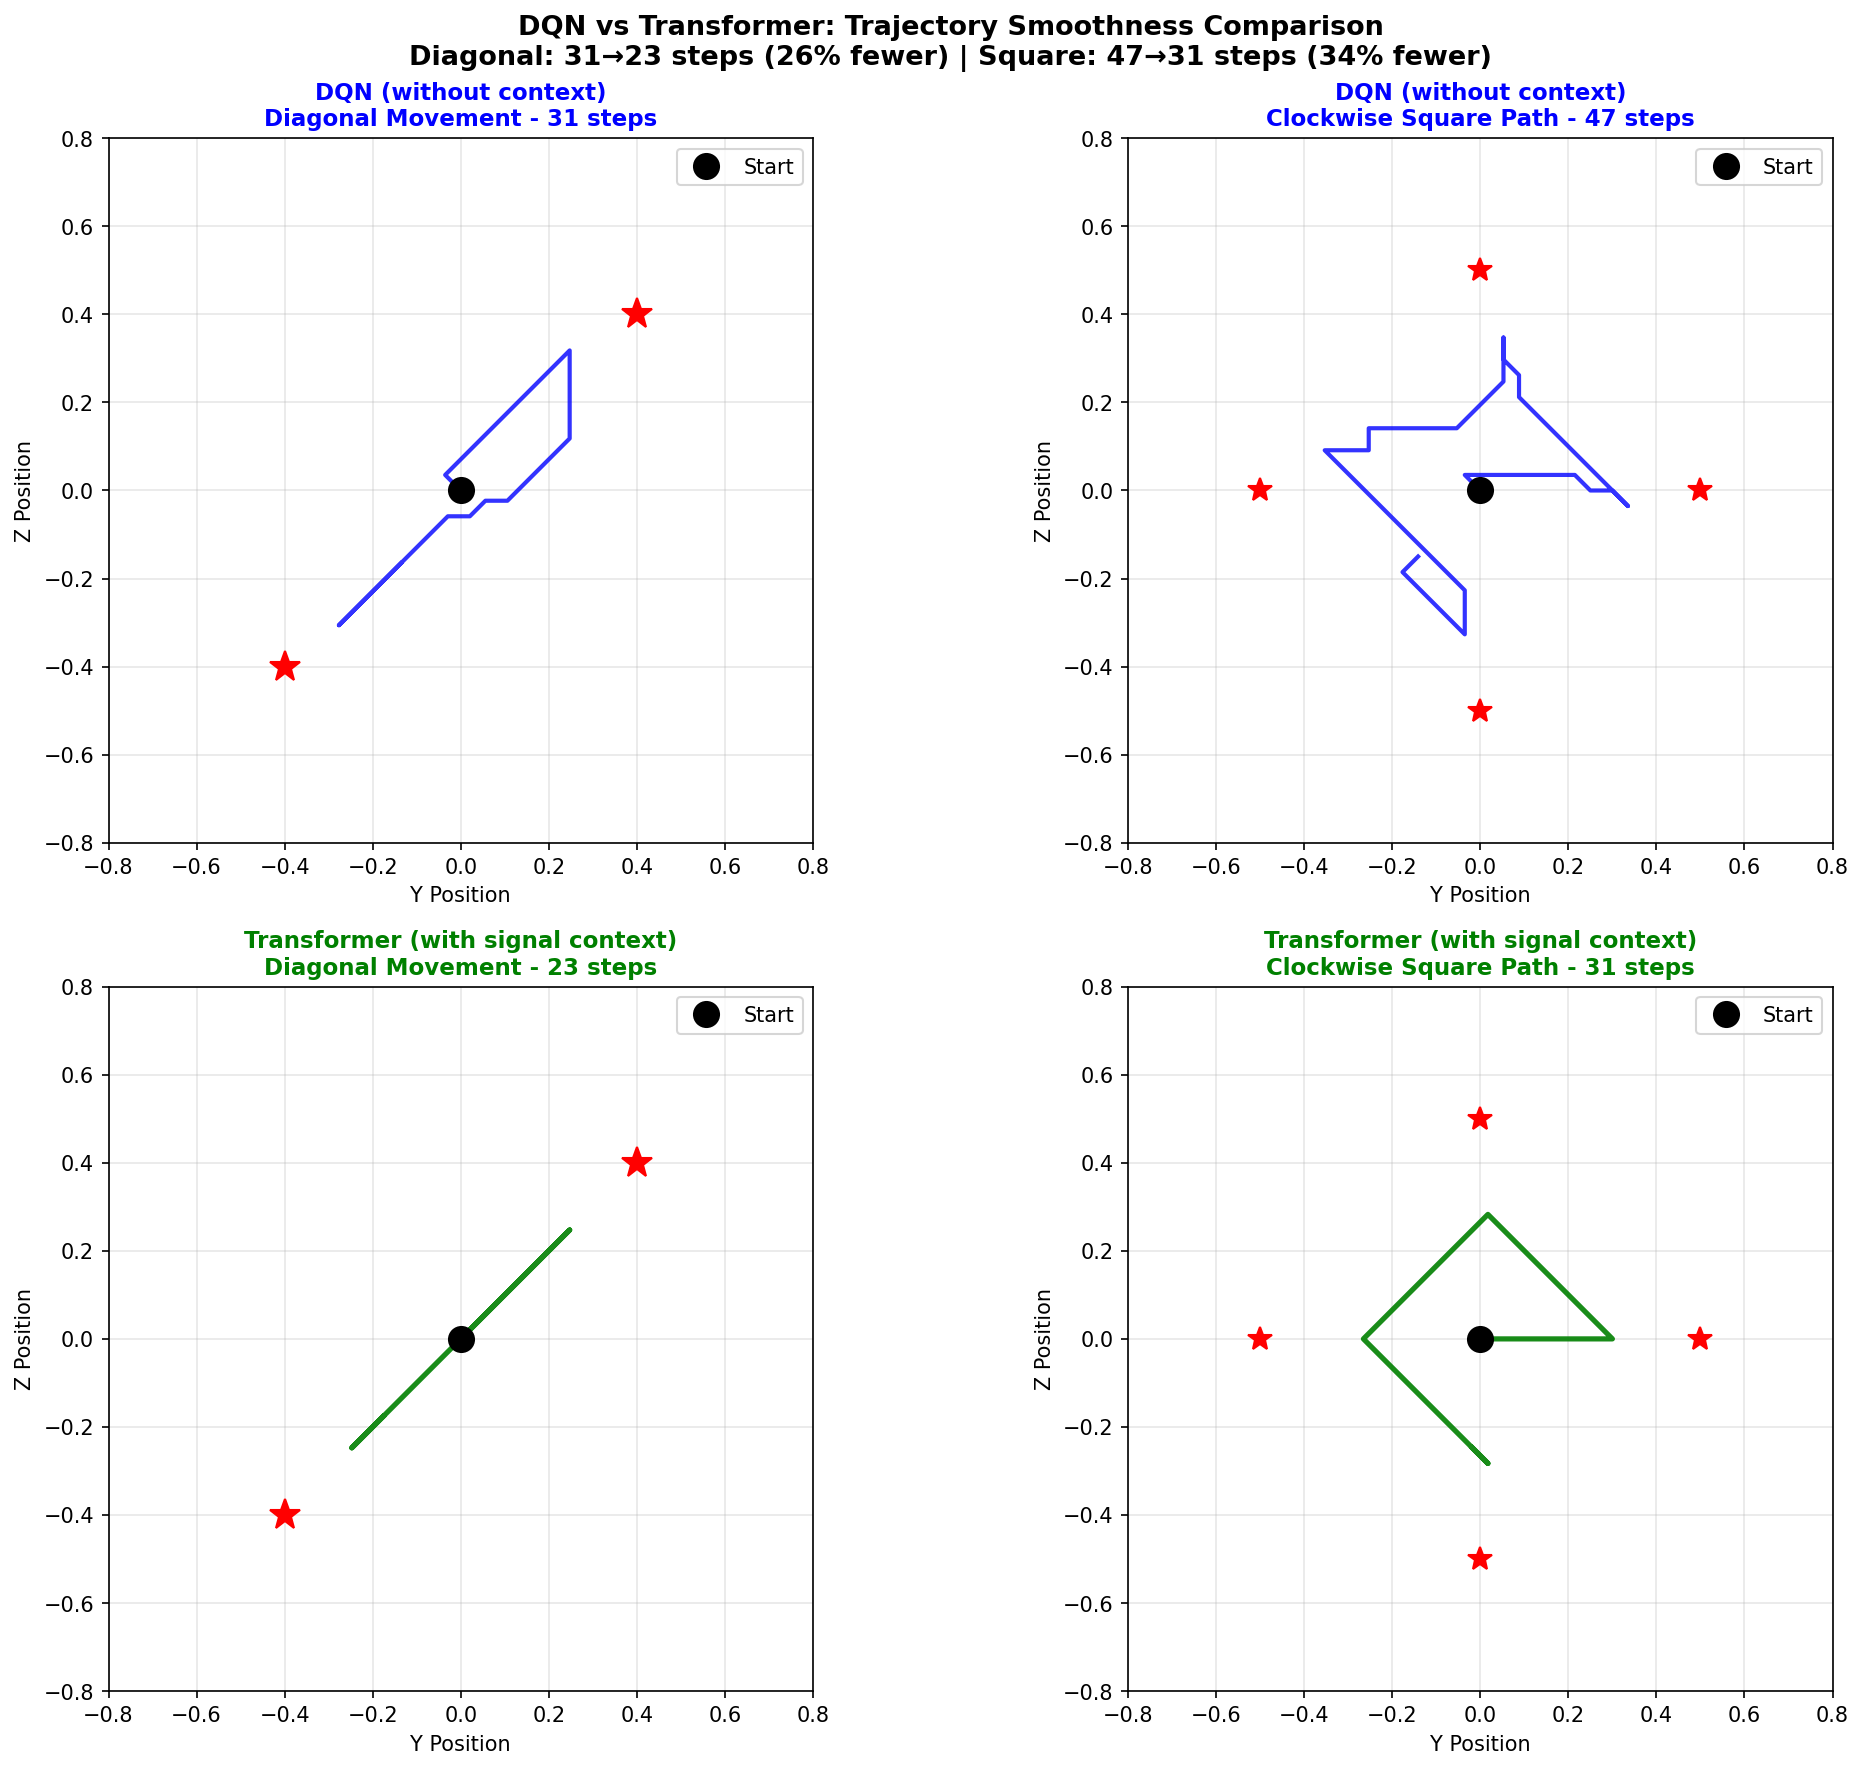
\includegraphics[width=\textwidth, height=0.8\textheight, keepaspectratio]{../outputs/comparison_dqn_vs_transformer_2cases.png}
    \end{columns}
\end{frame}

% ========== Slide 8: 综合对比图 ==========
\begin{frame}{Comprehensive Comparison}
    \begin{center}
        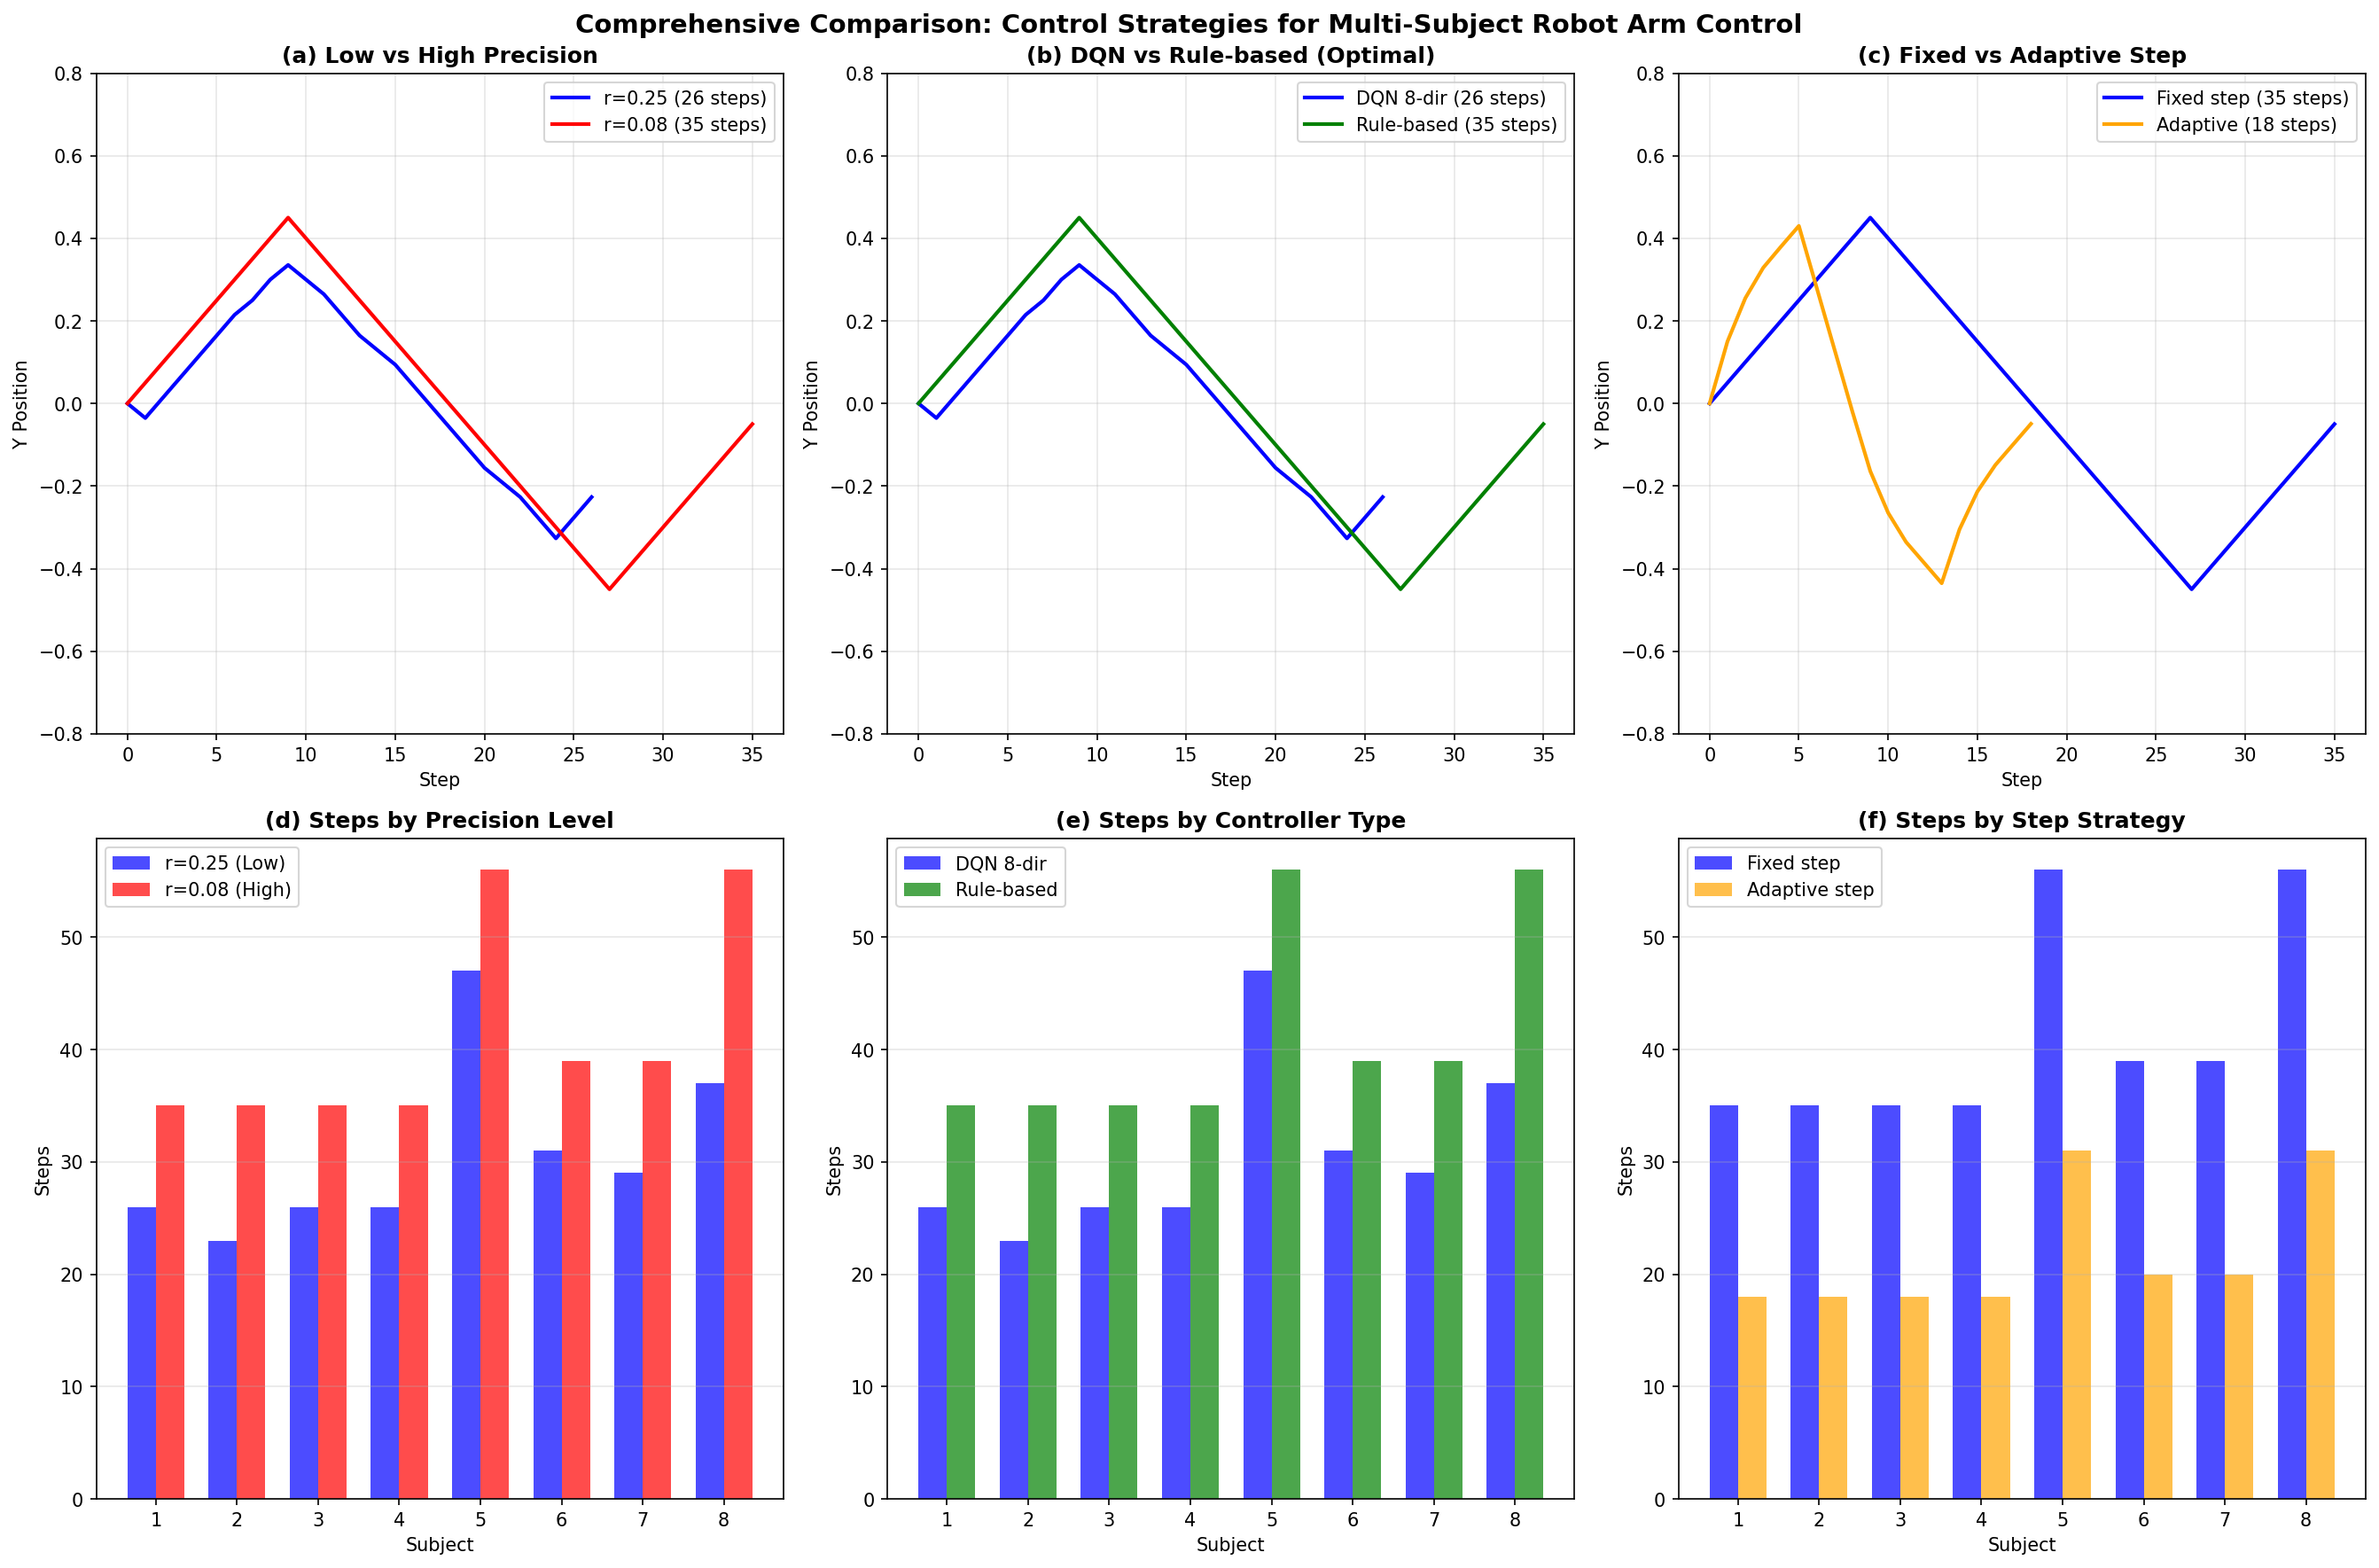
\includegraphics[width=0.92\textwidth, height=0.82\textheight, keepaspectratio]{../outputs/comprehensive_comparison.png}
    \end{center}
\end{frame}

% ========== Slide 8: Position vs Time 详细结果 ==========
\begin{frame}{Position vs Time Analysis}
    \begin{columns}[T]
        \column{0.5\textwidth}
        \textbf{Subject 1: Horizontal Sweep}
        
        
\includegraphics[width=\textwidth]{../outputs/multi_subject_sequence_adaptive/subject_1_position_vs_time.png}
        
        \column{0.5\textwidth}
        \textbf{Subject 5: Square Path}
        
        
\includegraphics[width=\textwidth]{../outputs/multi_subject_sequence_adaptive/subject_5_position_vs_time.png}
    \end{columns}
    
    \vspace{3mm}
    \textbf{Movement Patterns Tested:}
    \begin{itemize}
        \item Subjects 1-2: Horizontal sweep (left $\leftrightarrow$ right)
        \item Subjects 3-4: Vertical sweep (up $\leftrightarrow$ down)
        \item Subjects 5, 8: Square path (clockwise/counter-clockwise)
        \item Subjects 6-7: Diagonal sweep
    \end{itemize}
\end{frame}

% ========== Slide 9: 挑战与解决 ==========
\begin{frame}{Challenges \& Solutions}
    \begin{columns}[T]
        \column{0.5\textwidth}
        \begin{alertblock}{Challenges Encountered}
            \begin{itemize}
                \item Slow approach to target (35+ steps)
                \item Non-smooth trajectories with zigzag
                \item Blue line not reaching target star
            \end{itemize}
        \end{alertblock}
        
        \column{0.5\textwidth}
        \begin{exampleblock}{Solutions Applied}
            \begin{itemize}
                \item Adaptive step size: large far, small close
                \item 8-direction enables direct diagonal paths
                \item Reduced target\_radius: 0.25 $\rightarrow$ 0.08
            \end{itemize}
        \end{exampleblock}
    \end{columns}
    
    \vspace{5mm}
    \textbf{Step Size Strategy:}
    \begin{itemize}
        \item Far from target ($d > 0.5$): step = 0.15 (fast approach)
        \item Near target ($d < 0.17$): step = 0.05 (precise control)
        \item Result: 47.3\% faster convergence with same precision
    \end{itemize}
\end{frame}

% ========== Slide 10: 下周计划 ==========
\begin{frame}{Next Week's Plan}
    \begin{block}{Planned Tasks}
        \begin{enumerate}
            \item Physical robot arm testing with adaptive step size
            \item Real-time EEG classification integration
            \item Controller/Limiter: joint limit protection
            \item Smoother + Delay: reduce high-frequency jitter
        \end{enumerate}
    \end{block}
    
    \vspace{5mm}
    
    \begin{columns}[T]
        \column{0.5\textwidth}
        \textbf{Expected Deliverables:}
        \begin{itemize}
            \item Physical arm demo video
            \item Real-time BCI control demonstration
            \item Safety limit implementation
        \end{itemize}
        
        \column{0.5\textwidth}
        \textbf{Questions for Supervisor:}
        \begin{itemize}
            \item Is 0.08 target radius too strict for real robot?
            \item Should we add gripper open/close actions?
        \end{itemize}
    \end{columns}
\end{frame}

% ========== Slide 11: 时间线 ==========
\begin{frame}{Project Timeline}
    \begin{center}
    \resizebox{0.9\textwidth}{!}{%
    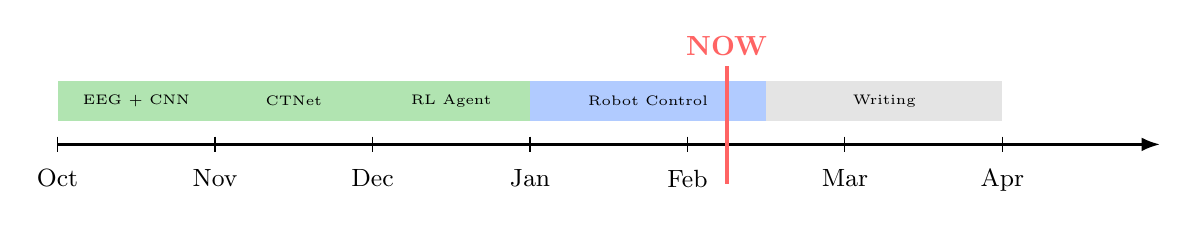
\begin{tikzpicture}
        \draw[thick, -Latex] (0,0) -- (14,0);
        
        \foreach \x/\month in {0/Oct, 2/Nov, 4/Dec, 6/Jan, 8/Feb, 10/Mar, 12/Apr} {
            \draw (\x, 0.1) -- (\x, -0.1);
            \node[below] at (\x, -0.2) {\small \month};
        }
        
        \fill[completed!50] (0, 0.3) rectangle (2, 0.8);
        \node at (1, 0.55) {\tiny EEG + CNN};
        
        \fill[completed!50] (2, 0.3) rectangle (4, 0.8);
        \node at (3, 0.55) {\tiny CTNet};
        
        \fill[completed!50] (4, 0.3) rectangle (6, 0.8);
        \node at (5, 0.55) {\tiny RL Agent};
        
        \fill[inprogress!50] (6, 0.3) rectangle (9, 0.8);
        \node at (7.5, 0.55) {\tiny Robot Control};
        
        \fill[pending!50] (9, 0.3) rectangle (12, 0.8);
        \node at (10.5, 0.55) {\tiny Writing};
        
        \draw[highlight, ultra thick] (8.5, -0.5) -- (8.5, 1);
        \node[highlight, above] at (8.5, 1) {\textbf{NOW}};
        
    \end{tikzpicture}}
    \end{center}
    
    \vspace{3mm}
    \textbf{Current Status:} On track
    
    \textbf{This Week's Achievement:} Multi-subject control with 47\% faster convergence
\end{frame}

% ========== Slide 12: Summary ==========
\begin{frame}{Summary}
    \begin{center}
    \Large
    \textbf{Key Achievements This Week}
    \end{center}
    
    \vspace{5mm}
    
    \begin{enumerate}
        \item \textbf{8-Direction Action Space}: Including diagonal movements for more natural control
        \item \textbf{High Precision Control}: Target radius reduced from 0.25 to 0.08 (3x more precise)
        \item \textbf{Adaptive Step Size}: 47.3\% faster target approach (330 $\rightarrow$ 174 steps)
        \item \textbf{8 Subject Patterns}: All subjects 100\% success rate
    \end{enumerate}
    
    \vspace{10mm}
    
    \begin{center}
    \textit{Output files: \texttt{outputs/multi\_subject\_sequence\_adaptive/}}
    \end{center}
\end{frame}

\end{document}
